\documentclass[doctor]{thesis}

% 定义本论文相关元信息
\def\thesisChineseBookName{论文题目}
\def\thesisEnglishBookName{English Thesis Title}



\title{\thesisChineseBookName}{\thesisEnglishBookName}

% \author{王稳}{Wang Wen}
% \advisor{赖生建\chinesespace 副教授}{Dr. Shengjian Lai}
% \school{物理电子学院}{School of Physical Electronics}
% \major{无线电物理}{Radio Physics}
% \studentnumber{201421040223}



\SetKwInOut{KIN}{输入}
\SetKwInOut{KOUT}{输出}







\begin{document}
% 插入封面
\thesisTitlePage

% 插入声明页
% \thesisDeclarationPage

% 中文摘要及关键词
\begin{chineseAbstract}
摘要内容


\chinesekeyword{关键词1;关键词2}
\end{chineseAbstract}

% 英文摘要及关键词
\begin{englishAbstract}
English Abstract.

\englishkeyword{Keyword 1; Keyword 2}
\end{englishAbstract}

%% 目录
\thesisContents

%% 主要符号对照表
\begin{thesisMainSymbol}
    $\mathbb{R}^d$        & $d$维Euclidean空间        \\
    $n$                    & 输入样本个数               \\
    $\mathbf{X}$           & 输入特征矩阵               \\
    $\mathbf{x}_i$         & 第$i$个样本的特征向量      \\
\end{thesisMainSymbol}

%% 缩略词表
\begin{thesisAcronyms}
    GNNs & Graph Neural Networks         & 图神经网络    \\
    GCN  & Graph Convolution Network     & 图卷积网络    \\
\end{thesisAcronyms}



\chapter{绪论}
\label{chapter_introduction}
\renewcommand{\headrulewidth}{0.4pt} % 在目录、符号表、缩略词表中去掉页眉下划线,这边需要恢复
%图片用\ref{XXX}引用
% \begin{figure}[!t]
%     \centering
%     \includegraphics[width=16.5cm]{XXX.pdf}
%     \caption{XXXXXX}
%     \label{chapter_sgae_fig_overview}
% \end{figure}

\section{研究背景与意义}
研究意义\citing{kolesnikov2019revisiting}。

\section{国内外研究现状}
内容。

\subsection{现状1}
内容。

\subsubsection{现状1.1}


\section{本文研究内容与贡献}

\textbf{1. 研究内容1}


\textbf{2. 研究内容2}



\section{本文组织结构}


\chapter{研究内容1}
研究内容。

\section{引言}


\section{算法框架}


\begin{algorithm}[!t]
    \caption{\textbf{XXXXX网络}}
    \KIN{输入}
    \KOUT{输出}% 输出
    算法
    \textbf{返回} $\mathcal{C}$
\end{algorithm}



\section{实验与分析}


\begin{table}[!t]
  \centering
  \caption{实验数据集统计信息}
  \begin{tabular}{*{5}{c}}
      \toprule
          数据集      & \#样本     & \#特征     & \#类别      & 数据类型 \\
      \midrule
          COIL20      & 1,440     & 1,024      & 20        & Object image \\
          COIL100     & 7,200     & 1,024      & 100       & Object image \\
      \bottomrule
  \end{tabular}
  \label{chapter_sgae_tab_datasets}
\end{table}

\begin{figure}[!t]
    \centering
    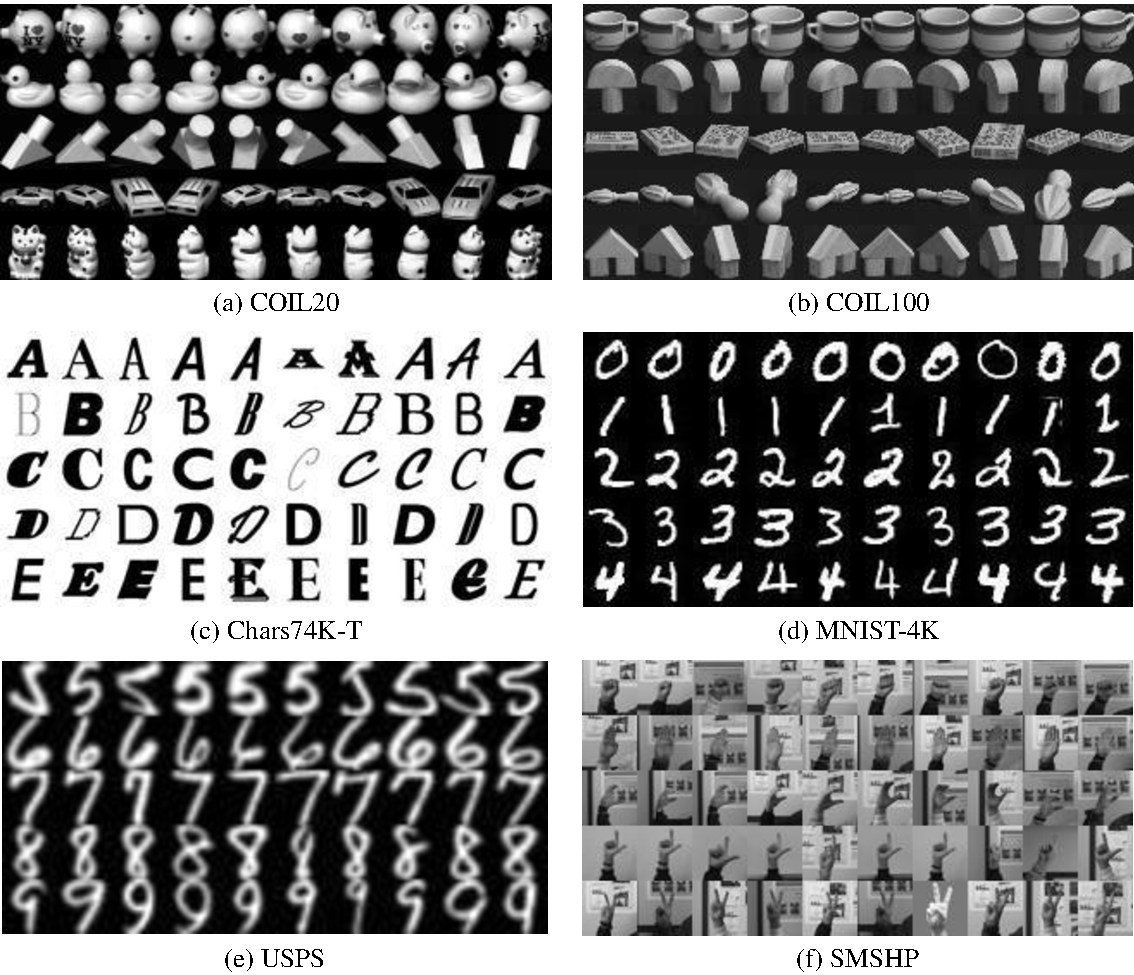
\includegraphics[width=16.5cm]{./figs/fig_data_visualization.pdf}\\
    \caption{部分实验图像数据集实例展示}
    \label{chapter_sgae_data_visualization}
\end{figure}








% 由于结论章节不能出现序号,这边重新定义一个命令
\thesisChapterConclusion
\chapter{}

\section{全文总结}



\section{后续工作展望}



% 参考文献                                    
\thesisbibliography{reference}

% 致谢
\begin{thesisAcknowledgement}
 致谢
\end{thesisAcknowledgement}

% 附录
\thesisappendix
\chapter{说明}
附录是对于一些不宜放在正文中,但有参考价值的内容,可以包括正文内不便列出的冗长公式推导,以备他人阅读方便所需的辅助性数学工具或表格,重复性数据图表,计算程序及说明。(如果没有附录可删除此章,导航窗格中鼠标右键章节标题有直接删除的菜单项) 
\section{测试}

% 简历
\begin{thesisResume}
    \begin{description}[labelsep=0pt, leftmargin=*]
        \item 姓\hspace{24pt}名:XXX
        \item 性\hspace{24pt}别:男
        \item 出生年月:XXXX年XX月
        \item 籍\hspace{24pt}贯:XX省XX市
    \end{description}

    \section*{\heiti\fontsize{14pt}{16.8pt}\selectfont 学习经历}
    \begin{description}[labelsep=0pt, leftmargin=*]
        \item 学士:软件工程,福州大学,2015.09-2019.06
    \end{description}

    \section*{\heiti\fontsize{14pt}{16.8pt}\selectfont 获奖情况}
    \begin{description}[labelsep=0pt, leftmargin=*]
        \item 2018年获福州大学硕士研究生中期优秀学业奖学金
    \end{description}
\end{thesisResume}

% 在学期间的研究成果及发表的学术论文
% \begin{thesisAccomplish}
%     \section*{\heiti\fontsize{14pt}{16.8pt}\selectfont 在学期间发表或在审论文:} 
%     \begin{enumerate}[labelindent=0pt, leftmargin=*]
%         \item \textbf{Shunxin Xiao}, Shide Du, Zhaoliang Chen, Yunhe Zhang, Shiping Wang*.
%         Dual Fusion-Propagation Graph Neural Network for Multi-View Clustering[J]. 
%         IEEE Transactions on Multimedia, 2023, DOI: 10.1109/TMM.2023.3248173.
%         \item \textbf{Shunxin Xiao}, Shiping Wang, Wenzhong Guo*. 
%         SGAE: Stacked Graph Autoencoder for Deep Clustering[J]. 
%         IEEE Transactions on Big Data, 2023, 9(1), 254-266.
%         \item \textbf{Shunxin Xiao}, Shiping Wang, Yuanfei Dai, Wenzhong Guo*. 
%         Graph Neural Networks in Node Classification: Survey and Evaluation[J]. 
%         Machine Vision and Applications, 2022, 33(1), 1-19.
%         \item Shiping Wang, \textbf{Shunxin Xiao}, William Zhu, Yingya Guo*.
%         Multi-View Fuzzy Clustering of Deep Random Walk and Sparse Low-Rank Embedding[J]. 
%         Information Sciences, 2022, 586, 224-238.
%         \item Huibin Lin, Shiping Wang, Zhanghui Liu, \textbf{Shunxin Xiao}, Shide Du, Wenzhong Guo*.
%         FMixAugment for Semi-supervised Learning with Consistency Regularization[C]//Chinese Conference on Pattern Recognition and Computer Vision, 2021, 127-139.
%         \item \textbf{Shunxin Xiao}, Huibin Lin, Conghao Wang, Shiping Wang, Jagath C. Rajapakse*.
%         Graph Neural Networks with Multiple Prior Knowledge for Multi-Omics Data Analysis[J].
%         IEEE Journal of Biomedical and Health Informatics. (Major Revision)
%         \item \textbf{Shunxin Xiao}, Huibin Lin, Jianwen Wang, Shiping Wang*.
%         Multi-Relation Augmentation for Graph Neural Networks[J].
%         IEEE Transactions on Emerging Topics in Computational Intelligence. (Under Review)
%     \end{enumerate}

%     \section*{\heiti\fontsize{14pt}{16.8pt}\selectfont 在学期间参与的科研项目:} 
%     \begin{enumerate}[labelindent=0pt, leftmargin=*]
%         \item 面向两岸热点事件的社交多媒体大数据协同感知与计算. 海峡联合基金重点项目. 项目编号: U1705262.
%         \item 先进Via-Pillar工艺下VLSI性能驱动多层布线算法研究. 国家自然科学基金面上项目. 项目编号: 61877010.
%     \end{enumerate}
% \end{thesisAccomplish}



\begin{thesisAccomplish}
    \section*{\heiti\fontsize{14pt}{16.8pt}\selectfont 在学期间发表或在审论文:} 
    \hspace{-26pt} 第一作者(1篇)
    \begin{enumerate}[labelindent=0pt, leftmargin=*]
        \item XXXXX[J]. 
        IEEE Transactions on Multimedia, 2023.
    \end{enumerate}
    第二作者(1篇)
    \begin{enumerate}[labelindent=0pt, leftmargin=*]
        \item XXXX[J]. 
        Information Sciences, 2022.
    \end{enumerate}
    共同作者(1篇)
    \begin{enumerate}[labelindent=0pt, leftmargin=*]
        \item XXXXX[C]//Chinese Conference on Pattern Recognition and Computer Vision, 2021.
    \end{enumerate}

    \section*{\heiti\fontsize{14pt}{16.8pt}\selectfont 在学期间参与的科研项目:} 
    \begin{enumerate}[labelindent=0pt, leftmargin=*]
        \item XXXXXXXXXXXXXXXXXXX
    \end{enumerate}
\end{thesisAccomplish}


\end{document}
